\documentclass[letterpaper]{article}
\usepackage{aaai}
\usepackage{times}
\usepackage{helvet}
\usepackage{courier}
\usepackage{graphicx}
\frenchspacing
\setlength{\pdfpagewidth}{8.5in}
\setlength{\pdfpageheight}{11in}
\pdfinfo{
/Title (Insert Your Title Here)
/Author (Put All Your Authors Here, Separated by Commas)}
\setcounter{secnumdepth}{0}  
 \begin{document}
% The file aaai.sty is the style file for AAAI Press 
% proceedings, working notes, and technical reports.
%
\title{Generate Handwritten Fonts \\ Based on StyleGAN}
\author{Chengruidong Zhang, Haoran Xi}
\maketitle

\section{Problem Statement}
Traditionally, making a font requires all images of the target character set. For example, a Chinese font designer needs to draw all letters, numbers and punctuation marks, as well as thousands of Chinese characters.
Obviously, these thousands of characters in the same font have some common features, such as stroke width, curvature, etc., to distinguish them from other fonts. This means we may be able to extract the necessary features from a small number of characters to generate all characters.
\begin{center}
    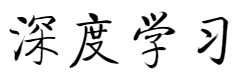
\includegraphics[]{proposal-fig-qiti.png}
    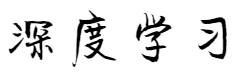
\includegraphics[]{proposal-fig-jinglei.png}

    Figure 1. Same characters in different fonts. 
\end{center}


\section{Target}
We will train a GAN model to extract the font style in the specified image and apply it to any character. For example, when we input the image of character "A" and the number 66 (the code of character "B"), it should output the image of "B" in the same font as the previous image of "A".
\begin{center}
    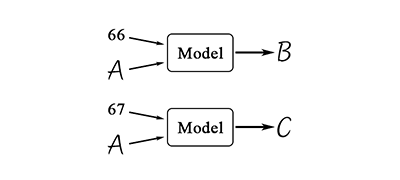
\includegraphics[]{proposal-fig-model.png}

    Figure 2. The function of our model. We are\\ going to generate all characters in this way.
\end{center}

\section{Related Works}
\subsection{Image Style Transfer Using CNN}
It is an algorithm that can separate and recombine the image content and style of natural images. A Convolutional Neural Network is trained to extract high level image information and produce new images of high perceptual quality that combine the content of an arbitrary photograph with the appearance of specified artworks. This work proves the feasibility of using CNN for image style transfer.
\subsection{StyleGAN}
StyleGAN is a GAN architecture with a style-based generator that receives additional inputs to adjust the style. It leads to an automatically learned, unsupervised separation of high-level attributes and stochastic variation in the generated images, and it enables intuitive, scale-specific control of the synthesis.
\\
While most of the style transfer papers focus on the images with human faces, we will focus on fonts instead.

\section{Brief Roadmap}
\subsection{Dataset}
The training set includes image sets converted from font files. System fonts such as Brush Script MT and Segoe Script can be used at the beginning. More handwritten fonts will be collected if necessary. We plan to start with English characters and numbers, and then then introduce Chinese characters.
\subsection{Building and Training Model}
We will use PyTorch to build the model and refer to the open source code on GitHub. To verify the algorithm, we can first use CPU to train a shallow model to handle small images of $32 \times 32$ pixels.

\section{Reference}
\smallskip \noindent
Leon, A. G., Alexander, S. E., and Matthias, B. 2016. Image Style Transfer Using Convolutional Neural Networks. \textit{CVPR}, pp. 2414-2423.

\smallskip \noindent
Tero, K., Samuli, L., and Timo, A. 2019. A Style-Based Generator Architecture for Generative Adversarial Networks. \textit{CVPR}, abs/1812.04948.

\bibliography{proposal-reference.bib}
\bibliographystyle{aaai}
\end{document}